
\chapter{ORGANIZATION}
      \section{History}
      Before joining their bachelor's program, they were self-motivated, reading business model books and always focused on starting a company. In the 3rd year of their bachelor's degree, they started their own company with a vision to contribute to society by teaching trending topics in technologies rather than being a client-service organization. Driven by a passion for entrepreneurship, they actively hosted various tech occasions. Currently, they are excited about bioinformatics research.
      
      \section{Objectives}
      The company has the following objectives:
      \begin{itemize}
        \item Initial goal: Empowerment of the youths in entrepreneurship
        \item Convert to a corporate company
        \item Create events so that youth can showcase their talents
        \item Research in bioinformatics
      \end{itemize}

      \section{Working of Organization}
      \subsection{Input}
        \begin{itemize}
          \item The company has made a clear short-term and long-term strategy to meet their goals.
          \item Urja Tech has a very few to none competitor in the valley.They have performed market analysis to follow current trends, analyse competitors and anticipate customer needs.
          \item Company has a detailed financial policy, performs regular financial reporting
          \item Following the demands and industrial trends, human resources are recruited and proper training and development programs are set for them along with compensation and benefits.
          \item The company has Legal Advisor for legal advice. needed.
          \item Urja Tech does minimal marketing as it has already made its presence in the valley.
          \item Company provides a friendly environment and proper environment for everyone to communicate.
      \end{itemize}
      \subsection{Output}
      The company provides the following services:
      \begin{itemize}
        \item Brand Guidaeline and Development
        \item Digital Marketing
        \item Event Management
        \item Technical Support for Business
        \item Cources on UTC(Urja Tech)
        \item Incubation and Enterpreneurship
        \item Human Resource Management
      \end{itemize}

      \section{Organizational Structure}
      Urja Tech has a hierarchical structure, which entails several layers of management that are in favor of a linear authority system. This arrangement promotes effective monitoring, making decisions, and assuring people are answerable if necessary. the detailed breakdown of the structure if shown below.
        \begin{enumerate}
           \item  \textbf{Top-Level Management}
            \begin{description}
                \item[\textbf{CEO:} ]  The CEO holds the highest authority within the company and is responsible for overall strategic planning, decision-making, and company oversight.
                
                \item \textbf{Directly Report to CEO:}
                
                \item[Legal Advisor: ]  The Legal Advisor handles all legal issues to make sure that the laws and rules are followed. They offer legal advice to the CEO as well as other departments, manage legal risks and administrate cases related to the company. 


                \item[Head Manager: ]  The Head Manager on the other hand is responsible for day to day operations in the company

                \item[CA(Chartered Accountant): ] The CA manages the financial operations of the company, including accounting, auditing, financial reporting, and budgeting. They ensure the financial health of the company and provide financial insights to support decision-making.
                 
            \end{description}
            
            \item \textbf{Middle Management}
            \begin{itemize}
                \item Under the \textbf{Head Manager:}
            \begin{description}
                \item[Manager: ] The Manager ensure that their team meets performance targets and sticks to company policies. 
                \item[System Admin: ] The System Admin manages the IT infrastructure, including system maintenance, network security, and technical support ensuring that the company’s technology resources are efficient and secure from attackers.
                \item[HR (Human Resources) Manager:] The HR department handles recruitment, training, employee relations, ensuring company finds the best talent.
            \end{description}
            \end{itemize}
            \item \textbf{Operational Level}
            \begin{itemize}
                \item Under the \textbf{Manager:}
            \begin{description}
                \item[Team Leader: ] The Team Leader supervise and guide their members to ensure the tasks and projects are completed efficiently and effectively meeting the requirements 
            \end{description}
            \end{itemize}
            \item \textbf{Execution Level}
            \begin{itemize}
                \item Under the \textbf{Team Leader:}
            \begin{description}
                \item[Team Members:] Team Members are basically responsible for the execution of the company's dat to dat operations, carry out specific tasks and projects as provided by the team leader.
            \end{description}
            \end{itemize}
        \end{enumerate}
        \begin{figure}[H]
          
          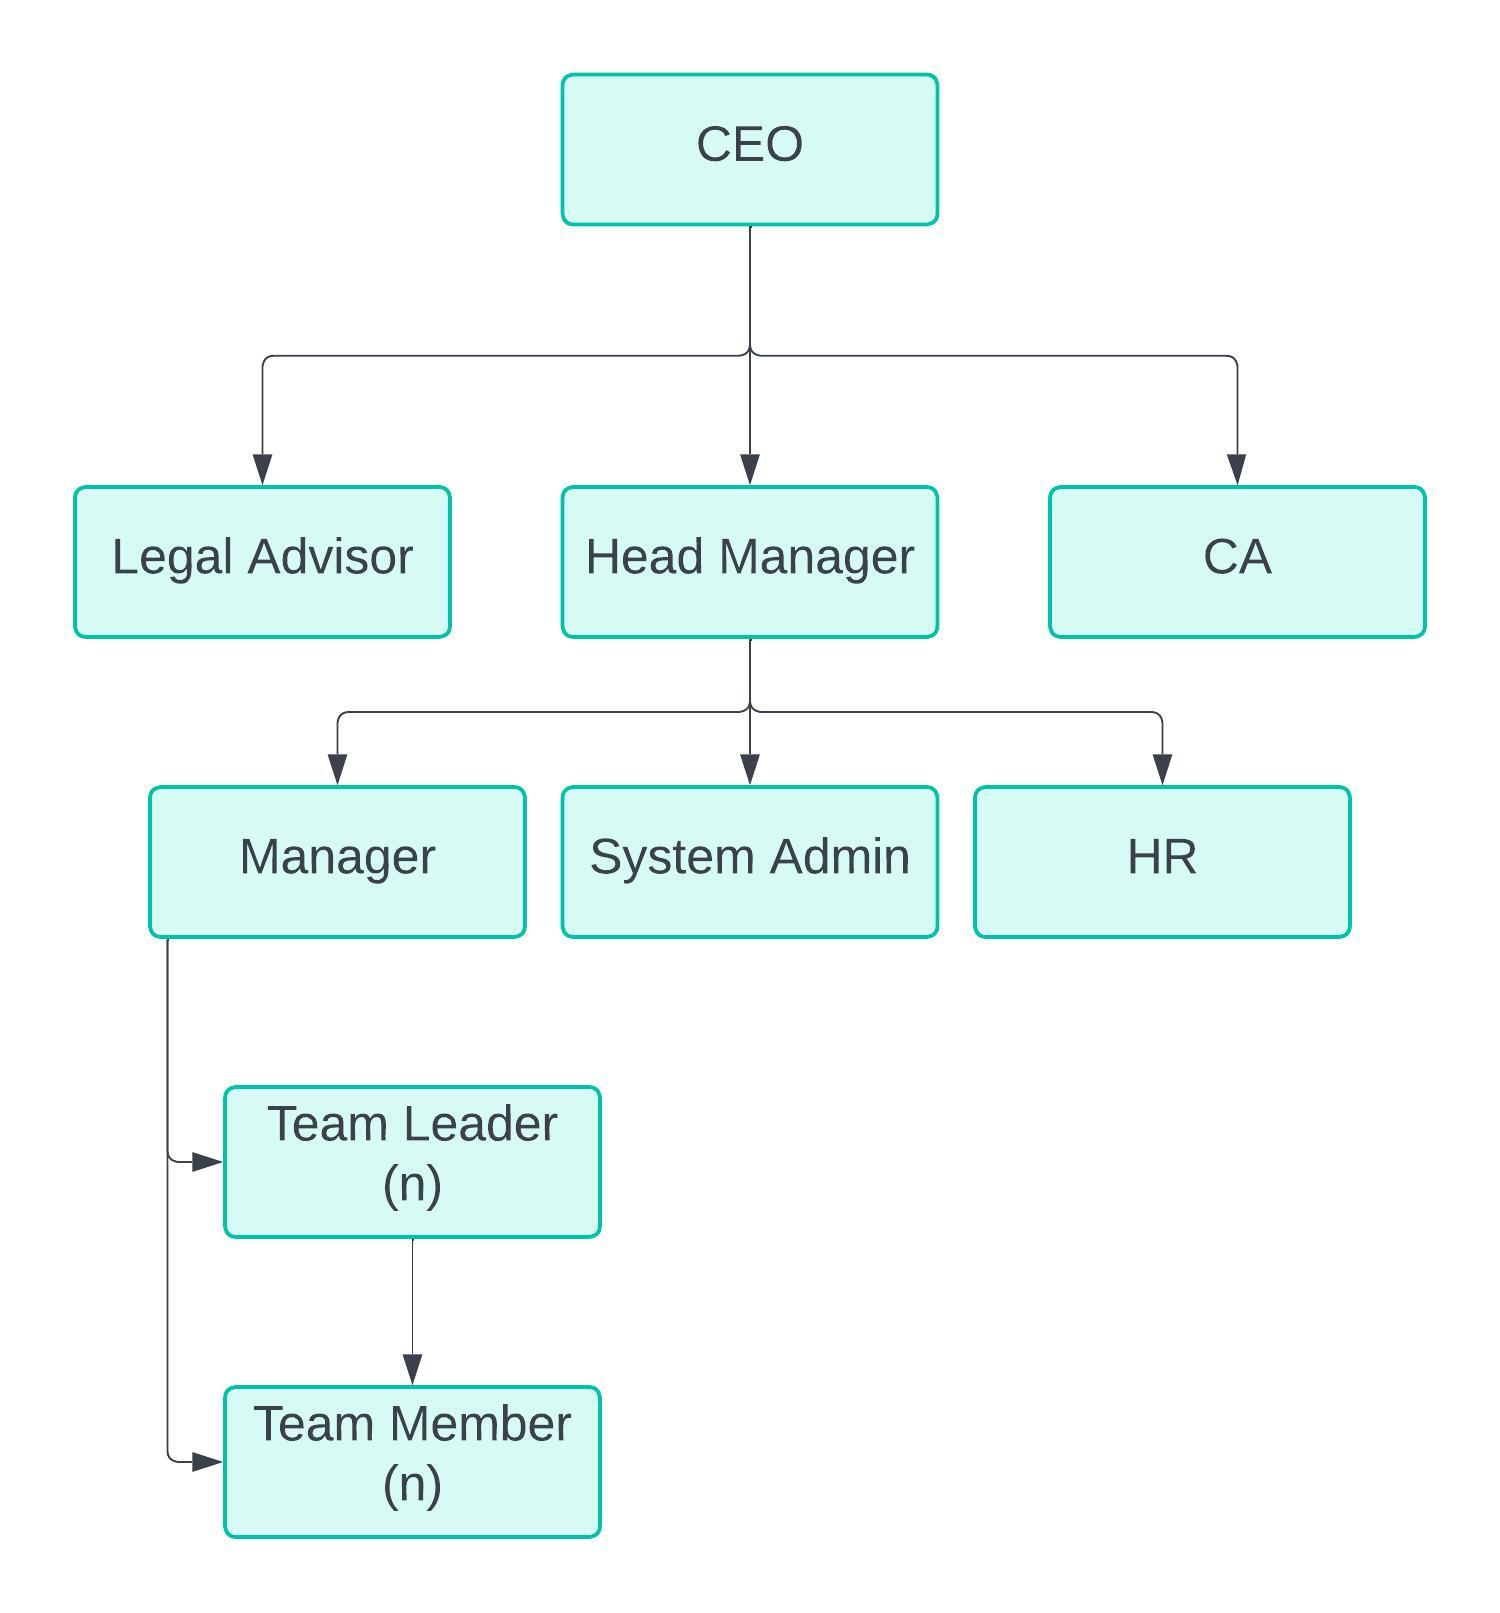
\includegraphics[width=\textwidth]{./Graphics/orgchart.jpeg}
          \caption{Organizational Structure of Urja Tech}
          \label{fig:orgchart}
        \end{figure}
        

      \section{Forms of Ownership}
     Essentially, this resembles a sole trader because the company relies on the form of its owner relationship where the company’s head, the chief executive officer is also the owner implying most control of the company concerns which have relationship with the management of such an organization. Furthermore, such a kind of structure is not very clear with the distinction between the owner and the business which implies that every decision and action made by the owner is taken into consideration as the personal life of the owner is of pertinent issue. thus he/she would be held accountable for any loss or obligation that business establishment would sustain. He/she runs and the other vice versa. Regardless that it operates as a sole trader, the above stated business would Still can have possibility with other firms if they are siblings In its current state of existence, supermarket still has the possibility of partnering with other companies. Sister organizations are separate legal entities which are legally affiliated to the same company. or ownership, commonly via a corporate group. Such exposures may be in the form of merg-er cooperation, binary or strategic partnerships, joint ventures, consignment, franchi- See more in section 2.2. ost complex forms, such as cooperation, joint venture or partnership, in which the different juridical and the operating structure of every entity remains unique and distinct from others. So, the sole pro- a few partners of proprietorship may combine with sister companies in certain circumstances such as-sharing. activities can only be defined as the acquisition and management of assets for the purpose of generating more revenues, increasing the markets, decreasing the costs or developing the innovations. Nevertheless, while in these affairs, the partners retain their organizational legal personalities yet affect one another’s. other to jointly realize their potential The various interests could refer to the following; Just what organisations may such partnerships involve to the level will be a function of collaborations between the firms and their novel reasons for the strategies. Sister companies – you might have heard about them are two or more companies that both entities are separate but can be affiliated with each other on the basis of having the same owner. Each of them is distinguished, in terms of its legal dimensions, from the other types of human relationships. The law and functioning also indicate that this organisational unit is still a separate company branch. Within this corporate setup the sole trader business might source some of its requirements from other related businesses for many reasons such as splitting the pie to get more clientele, cutting expenses in similar fashion, or coming up with new products. Each business maintains its face value identity (those personalities), but they cooperate and call as one big groups strength. The type of this kind of partnerships varies the nature of the relations between these companies and more to the point, how such companies establish their focus. objectives.
